\section{Experiments}\label{s:experiments}

In this section we demonstrate that our method is capable
of finding better experimental designs $S \subset [n]$
on data matrices $\X$ occuring in real-world applications.
We compare our method against the following references and recently proposed
methods for A-optimal design:
\begin{description}
    \item[Greedy bottom-up] adds an index $i \in [n]$ to the sample $S$
        maximizing the increase in A-optimality criterion
        \cite{greedy-supermodular,chamon2017approximate}.
       %  This method posesses well-understood theoretical bounds
       %  (however they
       % require additional assumptions on the matrix $\X$) and has strong
       %  empirical performance \cite{tractable-experimental-design}.

    \item[Our method (with SDP)] uses the efficient algorithms
        developed in proving Theorem~\ref{t:q2} to sample
        $\DPPreg{p}(\X,\A)$ constrained to subset size $k$
        with $p = w^*$, see \eqref{eq:sdp},
        obtained using a         recently developed first order convex cone solver called Splitting
        Conical Solver (SCS) \cite{o2016conic}.
        We chose SCS because it can handle the SDP constraints in
        \eqref{eq:sdp} and has provable termination guarantees, while
        also finding solutions faster \cite{o2016conic} than alternative
        off-the-shelf optimization software libraries such as SDPT3 and Sedumi.

    \item[Our method (without SDP)] samples $\DPPreg{p}(\X,\A)$ with uniform
      probabilities $p \equiv \frac{k}{n}$.
      % Compared to uniform and predictive length
      %   sampling, there is an additional DPP sampling overhead which is independent
      %   of sample size $k$ (but does depend on $d$).

    \item[Uniform] samples every size $k$ subset $S \subseteq [n]$
        with equal probability.

    \item[Predictive length] sampling \cite{zhu2015optimal} samples
        each row $\x_i$ of $\X$ with probability $\propto\|\x_i\|$.
\end{description}
Our experiments use data matrices $\X$ obtained from \texttt{libsvm} datasets
\cite{libsvm} (more details in Appendix~\ref{a:experiments}).

\subsection{Bayesian A-optimal design}

\Red{
    We first verify empirically that our method produces experimental
    designs which achieve good (lower) optimality criteria values, confirming
    the $(1+\epsilon)$-approximation guarantee provided by Theorem~\ref{t:q2}.
    Consistent with prior work in optimal Bayesian experimental design,
    we use the commonly adopted \citep{mariet2017elementary,chaloner1984optimal}
    A-optimality criterion
    $f_{\A}(\X_S^\top \X_S) = \tr \left((\X_S^\top \X_S + \A)^{-1}\right)$
}
The prior precision matrix is set to $\A = n^{-1} \I$,
and we consider sample sizes $k \in [d, 5d]$.
Each experiment is averaged over 25 trials and bootstrap 95\% confidence
intervals are shown.
% We provide open source implementations for efficient RDPP sampling
% and reproducing our results at \Red{TODO: fill in after blind review}.


\begin{figure}[htbp]
    \centering
    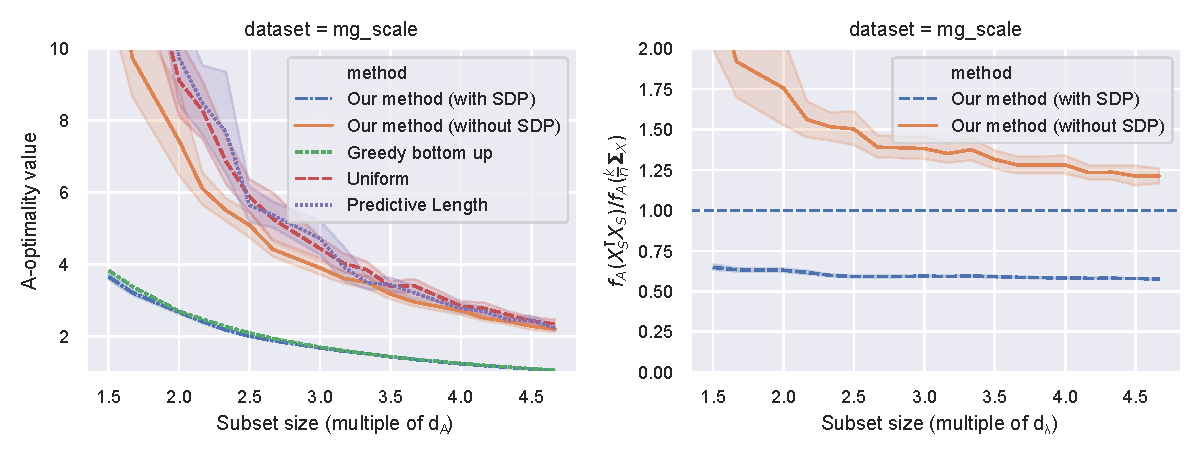
\includegraphics[width=0.5\textwidth,trim={0 0 10.2cm 0},clip]{../bayesian_figures/mg_combined.pdf}
     % 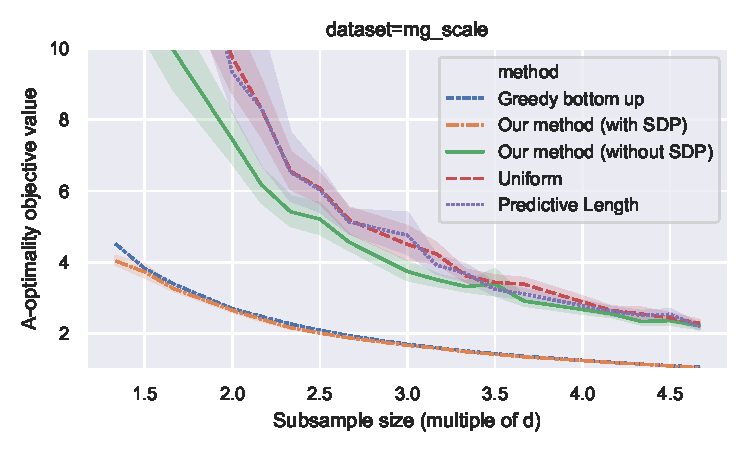
\includegraphics[width=0.51\textwidth]{../bayesian_figures/objectives-mg_scale-full.pdf}\hspace{-2mm}\nobreak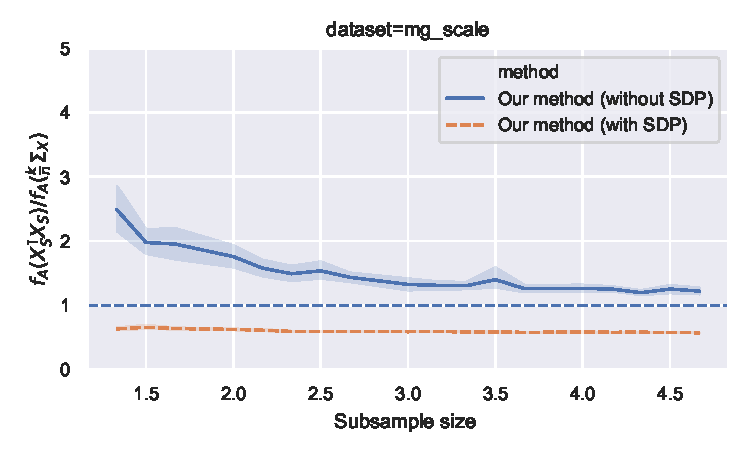
\includegraphics[width=0.51\linewidth]{../bayesian_figures/ratios-mg_scale.pdf}
    % 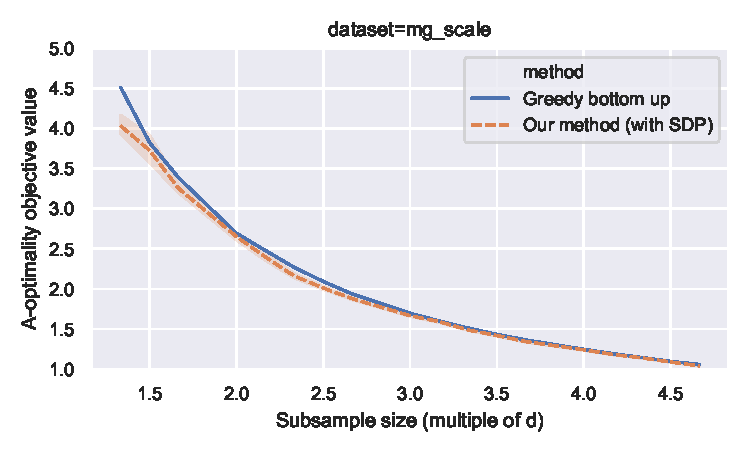
\includegraphics[width=0.49\textwidth]{../bayesian_figures/objectives-mg_scale-zoom.pdf}
    \caption{(left) A-optimality value obtained by the various methods on
        the \texttt{mg\_scale} dataset \cite{libsvm} with
        prior precision $\A = 10^{-5}\, \I$
    }
%         ,\quad (right)
% A-optimality value for our method (with and without SDP) divided by
% $f_{\A}(\frac kn\Sigmab_{\X})$, the baseline estimate suggested by Theorem \ref{t:q1}.
    \label{f:experiments}
\end{figure}

Figure~\ref{f:experiments} (left) reveals that our method (without SDP) is superior
to both uniform and predictive length sampling, producing designs which
achieve lower $A$-optimality criteria values for all sample sizes.
As Theorem~\ref{t:algorithm} shows that our method (without SDP) only differs
from uniform sampling by an additional DPP sample with controlled
expected size (see Lemma~\ref{l:size}), we may conclude
that adding even a small DPP sample can improve a uniformly sampled design.

Consistent with prior observations
\cite{chamon2017approximate,tractable-experimental-design}, the greedy bottom up
method achieves surprisingly good performance. However, if our method is used
in conjunction with an SDP solution, then we are able to match and
even slightly exceed the performance of the greedy bottom up
method. Furthermore, the overall run-time costs (see Appendix \ref{a:experiments})
between the two are comparable. As the majority of the runtime of our
method (with SDP) is occupied by solving the SDP, an interesting future direction
is to investigate alternative solvers such as interior point methods as well
as terminating the solvers early once an approximate solution is reached.

% Figure~\ref{f:experiments} (right) displays the ratio
% $f_{\A}(\X_S^\top \X_S)\, /\, f_{\A}(\frac{k}{n}\Sigmab_\X)$ for
% subsets returned by our method (with and without SDP). Note that the
% line for our method with SDP on
% Figure~\ref{f:experiments} (right) shows that the ratio never goes
% below 0.5, and we saw similar behavior across all examined datasets
% (see Appendix~\ref{a:experiments}). This evidence suggests that for
%     many real datasets $\opt$ is within a small constant factor of
%     $f_{\A}(\frac{k}{n}\Sigmab_\X)$, matching the upper bound of Theorem~\ref{t:q1}.
% As sample size $k \to n$, this should converge towards $1$ because $\X_S^\top
% \X_S \to \X^\top \X = \Sigma_X$.
% Across all datasets we examined, we see that this ratio is close to
% its asymptotic value of $1$. Similar to how condition
% numbers are the proper problem dependent constants in matrix inversion
% \cite{nocedal2006numerical}
% and $\tr (\frac{k}{n} \X^\top \X)^{-1}$
% is the problem-dependent constant which appear in results on non-Bayesian
% experimental design \feynman{Citation for this COLT paper?}, our results here
% suggest that $f_{\A}\left(\frac{k}{n} \X^\top \X\right)$
% is the proper problem-dependent constant for Bayesian optimal experimental
% design with a $k$ cardinality constraint.
% \feynman{Does this make sense?}

\subsection{Polynomial regression with low effective dimension}

\begin{figure}[htbp]
    \centering
    % \hspace{-0.55cm}
    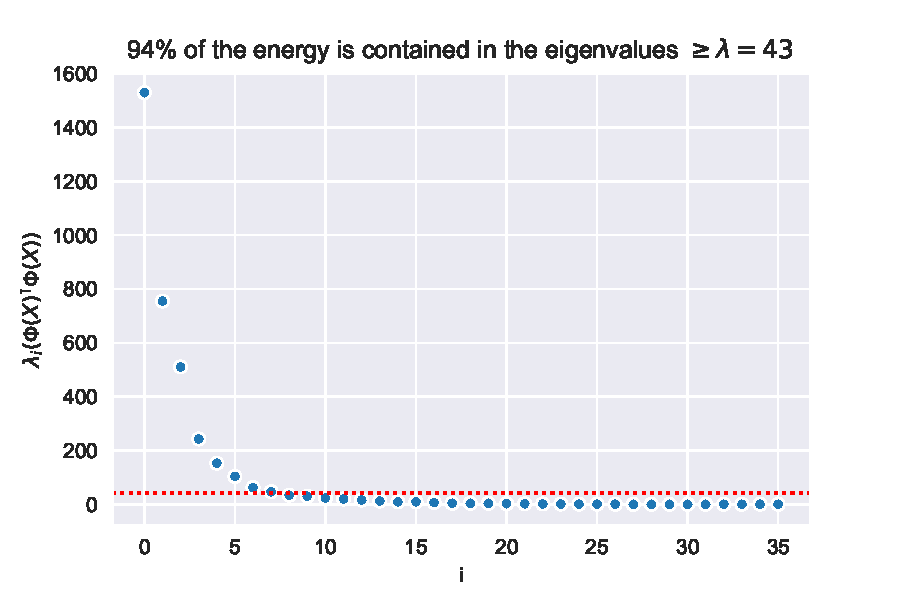
\includegraphics[width=0.5\textwidth]{Figures/screeplot.pdf}
    \caption{
        To determine the amount of regularization $\lambda$, a scree
        plot of the eigenvalues of the polynomially expanded
        covariance matrix $\Phi(X)^\top \Phi(X)$.
    }
    \label{fig:scree}
\end{figure}

\begin{figure}[htbp]
    \centering
    % \hspace{-0.85cm}
    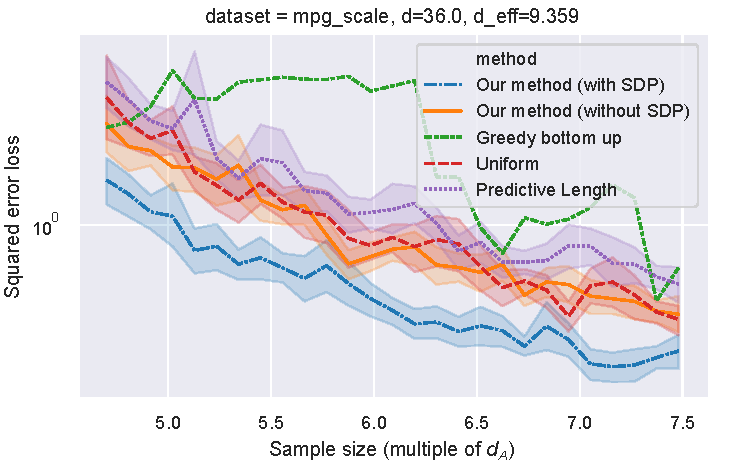
\includegraphics[width=0.5\textwidth]{Figures/mse_low_d_eff.pdf}
    \caption{Mean-squared error of subsampled least squares estimates
        for a degree 2 polynomial regression on \texttt{mpg\_scale} with
        $\lambda = 43$ (so the dimension $d = 36$ is much larger than the
        effective dimension $d_\A \approx 9.36$).
    }
    \label{fig:low_d_eff}
\end{figure}

\Red{
    As experimental design is oftentimes employed as a preprocessing
    step within a predictive modelling pipeline,
    we validate the practical utility of our algorithm by demonstrating
    superior performance for row subset selection in a polynomial
    regression task.  The \texttt{mpg\_scale} dataset \cite{uci-repository},
    which originally has $7$ features, is expanded using a degree 2 polynomial
    feature expansion to yield $d=36$ features.
    We choose $\A = \lambda \I$ where $\lambda = 43$ \feynman{Should we show
    scree plot Figure~\ref{fig:scree}?}, resulting in an effective dimension $d_\A \approx 9.35 \ll
    36 = d$.  Because $d_\A$ is more than three times smaller than $d$, the new
    theoretical results in this paper (Theroem~\cite{t:q1}) provide tighter
    guarantees than previous bounds which depended only on $d$.

    To perform polynomial regression, we run our algorithm on the
    data matrix with polynomial features to produce a $S \subset [n]$
    and subsequently form the subsampled least squares estimator
    $\hat{w}_S = \X_S^\dag y_S$. The quality of $\hat{w}_S$ is evaluated
    using mean-squared error from the full least squares estimator
    \begin{align}
        MSE &= \mathbb{E}_S\left[
            \|\hat{w}_S - \hat{w}_{[n]} \|^2
        \right]
    \end{align}
    Figure~\ref{fig:low_d_eff} illustrates our results over
    $100$ trials with $95\%$ confidence intervals. Our method outperforms all
    of the independent sampling (uniform and predictive length) methods,
    demonstrating the gains resulting from joint sampling.
    Also, contrary to Figure~\ref{f:experiments} we see that in terms
    of MSE our method is superior to the greedy bottom up method in
    almost all cases. This difference may be due to
    smaller effective dimension or because of the difference between
    A-optimality and MSE, and we plan to further investigate this in
    upcoming work.
}

